\subsubsection{Basic Data Analysis}

\begin{figure}[H]
	\centering
	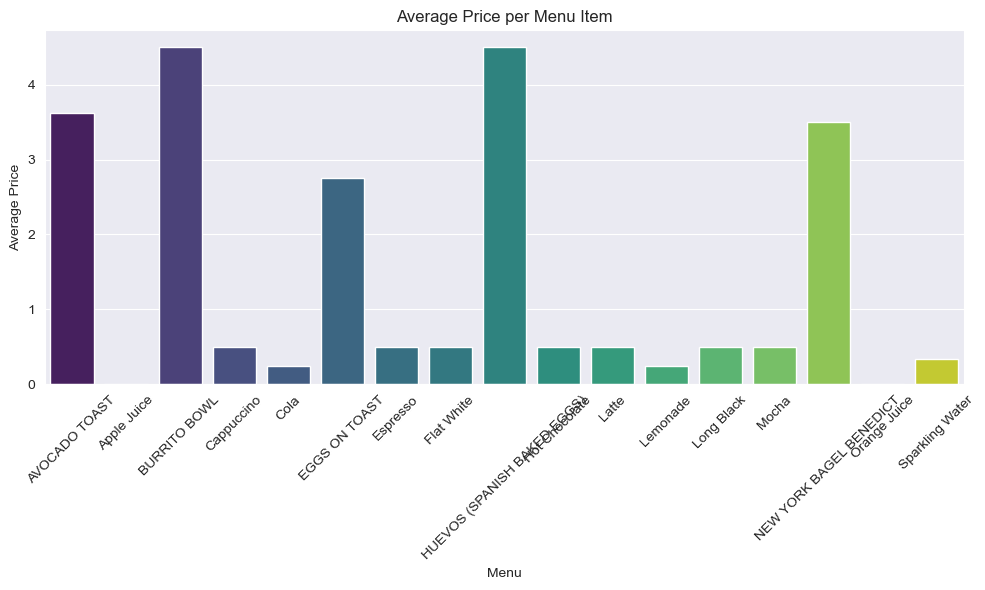
\includegraphics[width=0.8\textwidth]{assets/basic/average price per menu per item.png}
	\caption{Average price per menu per item}
	\label{fig:average_price_per_menu_per_item}
\end{figure}

The average price per menu item depicted in this figure suggests that the overall cost of dining at this establishment is relatively affordable, with prices ranging from \$0.50 to \$4.5. It's worth noting that the lowest price point of \$0.50 does not include water, which is complimentary.

\begin{figure}[H]
	\centering
	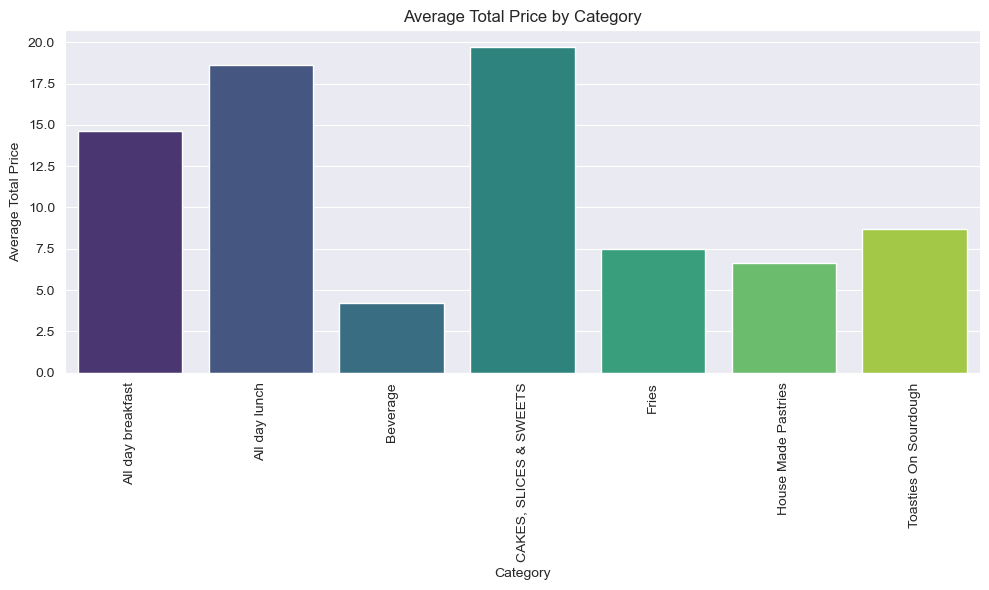
\includegraphics[width=0.8\textwidth]{assets/basic/average total price by category.png}
	\caption{Average total price by category}
	\label{fig:average_total_price_by_category}
\end{figure}

The analysis of the price distribution across various categories reveals a notable disparity between the highest-priced items, specifically those classified under "cake and bakery," and the lowest-priced items, which fall within the "Beverage" category. This observation suggests that despite the significant difference in prices, consumers continue to purchase products from both categories, indicating a strong demand for these goods.

\begin{figure}[H]
	\centering
	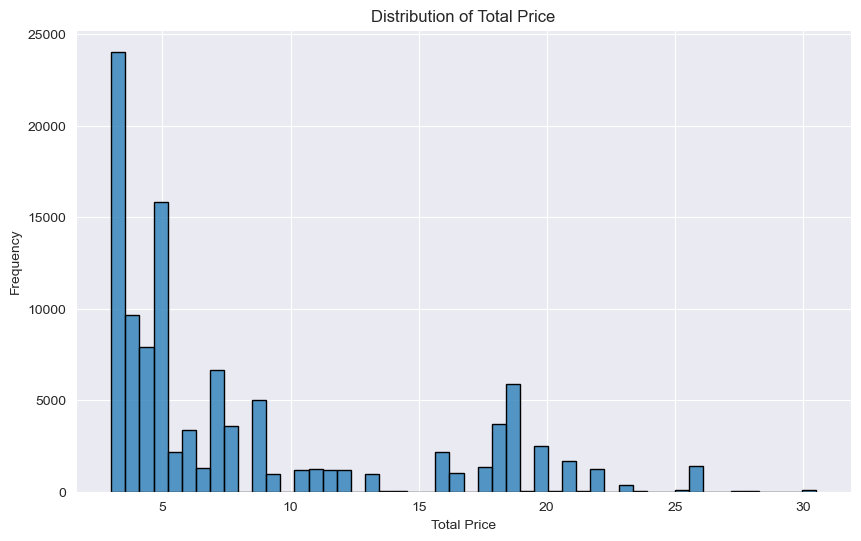
\includegraphics[width=0.8\textwidth]{assets/basic/distribution of total price.png}
	\caption{Distribution of total price}2
	\label{fig:distribution_of_total_price}
\end{figure}

As depicted in the accompanying figure, the total price distribution reveals a pronounced concentration of purchased items within the price range of \$3 to \$10, with a notable tail extending up to \$31 or more per item. This pattern suggests that the majority of consumers are inclined towards purchasing products at moderate prices, while a smaller proportion is willing to invest in higher-priced items.

\begin{figure}[H]
	\centering
	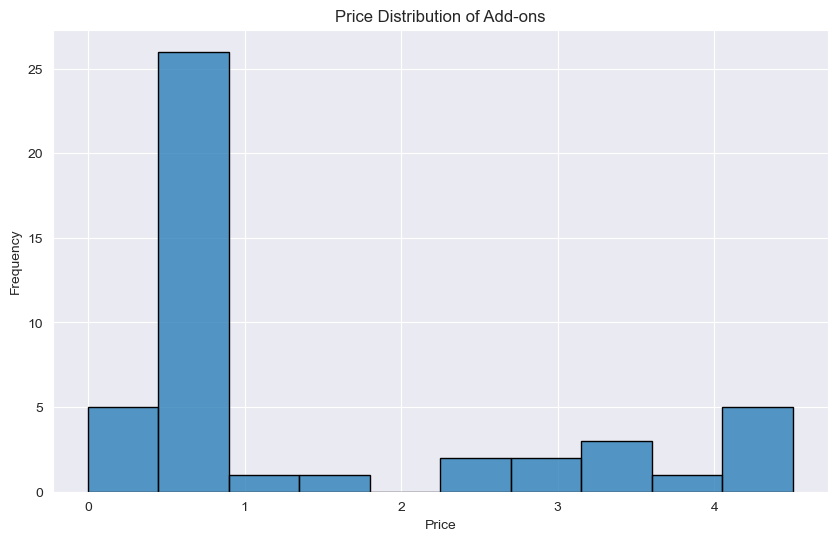
\includegraphics[width=0.8\textwidth]{assets/basic/price distribution of add ons.png}
	\caption{Price distribution of add-ons}
	\label{fig:price_distribution_of_addons}
\end{figure}

As illustrated in the accompanying figure, the price distribution of add-ons reveals a dominant pattern, with the majority of purchased items falling within the price range of \$0 to \$5 or more per item. This trend suggests that consumers are generally inclined towards acquiring low-cost or free add-ons, while a smaller proportion is willing to invest in higher-priced options.














